\providecommand{\main}{..}
\documentclass[../cmpe-251-project-report.tex]{subfiles}
\externaldocument{5-predictors}

\begin{document}
  \chapter{Properties of the Dataset}
  \label{ch:dataset-properties}
  The dataset has no missing attribute values, which avoids the challenge of having to fill in or compensate for any missing values. In lieu of this, practically all numerical attributes in the dataset are unimodally distributed with a positive skew in the range of 1 to 7.5. For instance, a histogram of the Product Related attribute values seen in \cref{fig:attribute-distribution} shows the positively skewed distribution of the attribute.
  \begin{figure}
    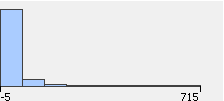
\includegraphics{product-related-distribution.png}
    \caption{Histogram of the Product Related attribute values.}
    \label{fig:attribute-distribution}
  \end{figure}
  The significance of the distribution increases for the target attribute we want to predict. The Revenue attribute has two classes, TRUE and FALSE, representing whether a visitor eventually bought an item from Nozama's website. Of the \num{12330} records in the dataset, \qty{84.5}{\percent} of the values for Revenue are FALSE, which implies that any predictor could easily attain a prediction accuracy of \qty{84.5}{\percent} if it always predicted Revenue to be false. Therefore, the evaluation of predictors should factor this in as a minimum prediction accuracy to achieve.

  Given that both the prediction attributes and the target attribute have similar distributions, the correlation between the attributes were observed next. From \cref{fig:rank-correlation}, two relatively significant correlations for Exit Rates and Page Values can be observed in relation to revenue. One should expect to see that Exit Rates and Page Values play in important role in predicting the target attributes, which will be explored further in later steps of the analysis.
  \begin{figure}
    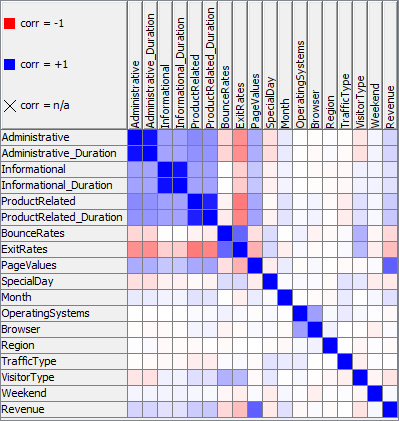
\includegraphics{rank-correlation.png}
    \caption{Rank correlation matrix of the attributes.}
    \label{fig:rank-correlation}
  \end{figure}
  As far as why the data is distributed this way, one could reason that a majority of visitors to Nozama's website tend to not interact much with it and don't make any purchases, leading to the high number of low values for each numerical attribute.
\end{document}
